%
% The first command in your LaTeX source must be the \documentclass command.
\documentclass[sigconf]{acmart}

% Disable the extra information at the foot at first page for better viewing experience for a normal document.
\settopmatter{printacmref=false} % Removes citation information below abstract
\renewcommand\footnotetextcopyrightpermission[1]{} % removes footnote with conference information in first column
\pagestyle{plain} % removes running headers

%
% defining the \BibTeX command - from Oren Patashnik's original BibTeX documentation.
\def\BibTeX{{\rm B\kern-.05em{\sc i\kern-.025em b}\kern-.08emT\kern-.1667em\lower.7ex\hbox{E}\kern-.125emX}}
    
% Rights management information. 
% This information is sent to you when you complete the rights form.
% These commands have SAMPLE values in them; it is your responsibility as an author to replace
% the commands and values with those provided to you when you complete the rights form.
%
% These commands are for a PROCEEDINGS abstract or paper.
%\copyrightyear{2018}
%\acmYear{2018}
%\setcopyright{acmlicensed}
%\acmConference[Woodstock '18]{Woodstock '18: ACM Symposium on Neural Gaze Detection}{June 03--05, 2018}{Woodstock, NY}
%\acmBooktitle{Woodstock '18: ACM Symposium on Neural Gaze Detection, June 03--05, 2018, Woodstock, NY}
%\acmPrice{15.00}
%\acmDOI{10.1145/1122445.1122456}
%\acmISBN{978-1-4503-9999-9/18/06}

%
% These commands are for a JOURNAL article.
%\setcopyright{acmcopyright}
%\acmJournal{TOG}
%\acmYear{2018}\acmVolume{37}\acmNumber{4}\acmArticle{111}\acmMonth{8}
%\acmDOI{10.1145/1122445.1122456}

%
% Submission ID. 
% Use this when submitting an article to a sponsored event. You'll receive a unique submission ID from the organizers
% of the event, and this ID should be used as the parameter to this command.
%\acmSubmissionID{123-A56-BU3}

%
% The majority of ACM publications use numbered citations and references. If you are preparing content for an event
% sponsored by ACM SIGGRAPH, you must use the "author year" style of citations and references. Uncommenting
% the next command will enable that style.
%\citestyle{acmauthoryear}

%
% end of the preamble, start of the body of the document source.
%\setcopyright{none}
\begin{document}

%
% The "title" command has an optional parameter, allowing the author to define a "short title" to be used in page headers.
\title{Paper Review CS846, Jan. 16\\
Software analytics and its application in practice}

%
% The "author" command and its associated commands are used to define the authors and their affiliations.
% Of note is the shared affiliation of the first two authors, and the "authornote" and "authornotemark" commands
% used to denote shared contribution to the research.
\author{Wenhan Zhu (Cosmos)}
\email{w65zhu@uwaterloo.ca}
\affiliation{%
  \institution{University of Waterloo}
  \city{Waterloo}
  \country{Canada}
}

%
% The abstract is a short summary of the work to be presented in the article.
\begin{abstract}
    This week's paper reviewed here are: {\bf Software analytics and its application in practice} by {\it Dongmei Zhang, Tao Xie} and {\bf No silver bullet: Essence and accidents of software engineering} by {\it Fred Brooks}. 
    
    {\it Zhang and Xie} talked about the aspects of software analytics and how to approach data and apply the results in practice. {\it Brooks} article expressed his view on the problem of solving software related issues and his view on that the problem will always exists and there will not be a method that will end this issue.
\end{abstract}

%
% Keywords. The author(s) should pick words that accurately describe the work being
% presented. Separate the keywords with commas.
%\keywords{paper review}

%
% A "teaser" image appears between the author and affiliation information and the body 
% of the document, and typically spans the page. 
%\begin{teaserfigure}
  %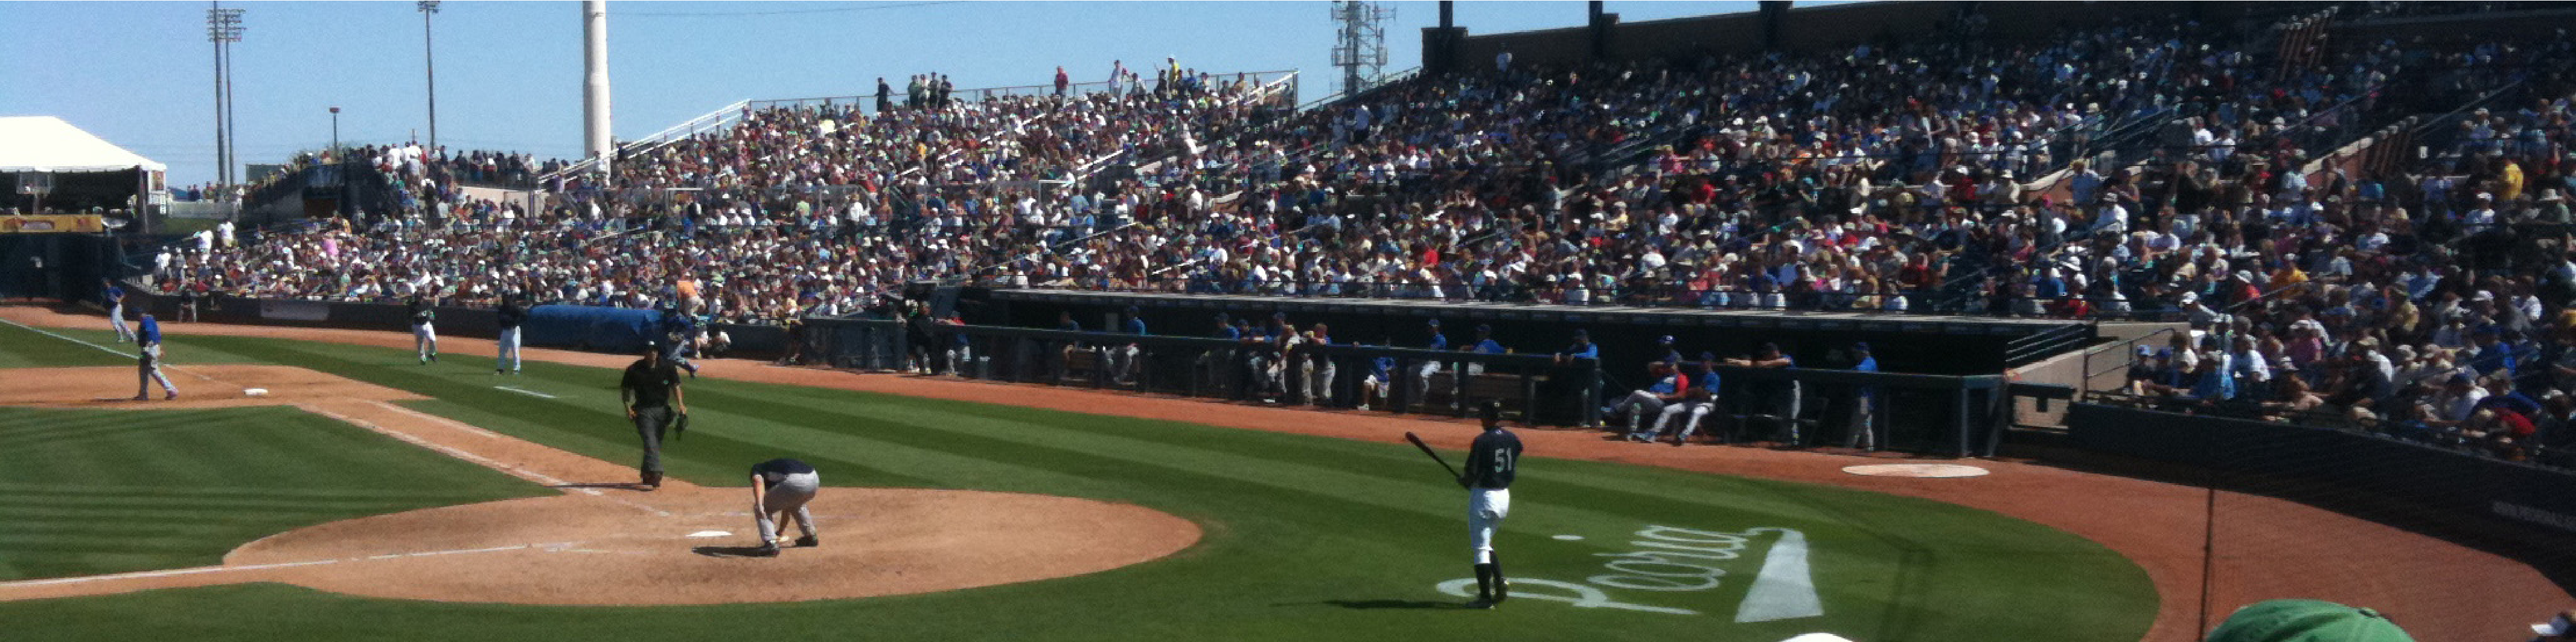
\includegraphics[width=\textwidth]{sampleteaser}
  %\caption{Seattle Mariners at Spring Training, 2010.}
  %\Description{Enjoying the baseball game from the third-base seats. Ichiro Suzuki preparing to bat.}
  %\label{fig:teaser}
%\end{teaserfigure}

%
% This command processes the author and affiliation and title information and builds
% the first part of the formatted document.
\maketitle

\section{Summary}
The chosen combined readings address different problems in the field of software engineering. {\it Zhang and Xie} talked about the different perspectives of software analytics and their recent experiences in applying software analytics in practice. They categorized software analytics in 6 perspectives, research topics, target audience input, output, technology pillars and connections to practice. The first 4 perspectives are very straight forward. The later two are further discussed in detail by the authors by they belong to the perspectives of software analytics. Technology Pillar is the techniques used by software analytic. These techniques evolve over time and the technologies have their own advantages and disadvantages. There are active research to improve the used technologies. Connection to practice describes the perspective that software analytics are tied with four real elements in the scope of data, problems, users and tools. The authors gave some valuable learnings from putting software analytics in action. The most important part is to identify the essential problem then have an active development feedback cycle to iteratively create solutions. Finally it is essential for the researchers to have a deep understanding of the domain of the subject to perform the analytic. 

{\it Brooks} article has many of his views of the software engineering world a few decades ago. Many of his predictions were true and some of his insights are still very valuable in today's standard. {\it Brooks} made a metaphor of software evolving into an unmanageable mess as people turning into werewolves. However, unlike the folklore, there are no silver bullet to the problem of software artifacts. He decomposed software engineering to two parts, one is the artifact or side-effects of current software engineering tools that is tied to a specific set of circumstances and often does not apply between programming languages and practices. The other is the essential problems that is unavoidable as long as we are still producing software. He gave his view on the advancements of technology at the time and they could not solve essence problems of software engineering. In the end, he advocates for the need for great designers of problems. He believes that it is the great designers that creates produces great software.

\section{Thoughts}
Many idea from {\it Zhang and Xie} seem to originates from the open source community and the agile development protocol. The description about the learning they found from software analytics in practice seems to suggest that the software analytic itself is a form of software development. I think the perspectives they gave captures the scope of software analytics and shows how it is used and what information it needs and provides in a generic setting. 

I really liked {\it Brooks} paper. It showed great insight on what he though about software engineering. His arguments about object oriented programming predicted the problems it solved and the problems it couldn't address. But I think there are still some points that he missed. One is the graphical user interface. He failed to predict convenience graphical user interface brought to everyday computing and more people can learn programming more easier then before. But he did see that "smart" programming environments (IDE's of today) does not solve essence problems. From my point of view, I agree that these tools only scratch itches of the development process but does not address essential problems on software engineering. Large system still needs to build from ground up and the design is more important than the smaller details. And based on the time the article was published, the current open source development model did not appear in the software engineering world. By looking at history, it seems to me that open source project was able to introduce many new ideas and give solutions to some of the old software engineering problems. With the involvement of more people is seems like a ecosystem that wasn't something imaginable at the time given that most software are still hardware specific. Many historical affects are still valid today that software like {\it xterm} needs to support terminal standards that are decades old and probably no one still uses them.

I think the open source community really introduced a new way to look at software development. Compared to the traditional way, open source development have contributors that will work on problems that they want to solve and software will evolve to what people need. So instead of having to evaluate what software to develop and what features people what, in the open source world people will decide on their own. And in such process, the essence part of software engineering in my mind follows the pattern of natural evolution such that the good ones will stay and the bad ones will become irrelevant or extinct. 

\section{Ratings}
I would give {\it Zhang and Xie}'s paper a 3 out of 5. It talks about their view on software analytics and their learnings of applying it in practice. However, I don't find it giving me detailed understanding of what could software analytics provide when used in practice.

I really enjoyed {\it Brooks} article. I would rate it a 5. It's an excellence paper that discusses many ideas which are still applicable today. 

\section{Questions}
I've attended Daniel Berry's talk on his view of software engineering. He mentioned that in the beginning of time, people believed that by designing better programming languages people could produce good software. But it failed and people eventually realized that it's a own field of study of how to produce good software. Then he moved to the study of requirement engineering which works on how to extract specific requirements from language descriptions to software engineering problems which can then be done by software engineers. As of today we still do not have a good metric to tell good software from bad ones. And the type of software is also shifting, from business practices from the early days to mobile apps about a decade ago and now web applications. In these context the type of software changes and so does many things. Do essence also shift in this manner? A concrete example would be it's probably a huge problem in the past where memory is wasted but now as long as there are no memory leak and the magnitude of memory usage is still on the same level no one would care if it takes more memory as long as it gets the job done.

% The next two lines define the bibliography style to be used, and the bibliography file.

\end{document}
